% Created by tikzDevice version 0.12 on 2019-04-30 13:25:14
% !TEX encoding = UTF-8 Unicode
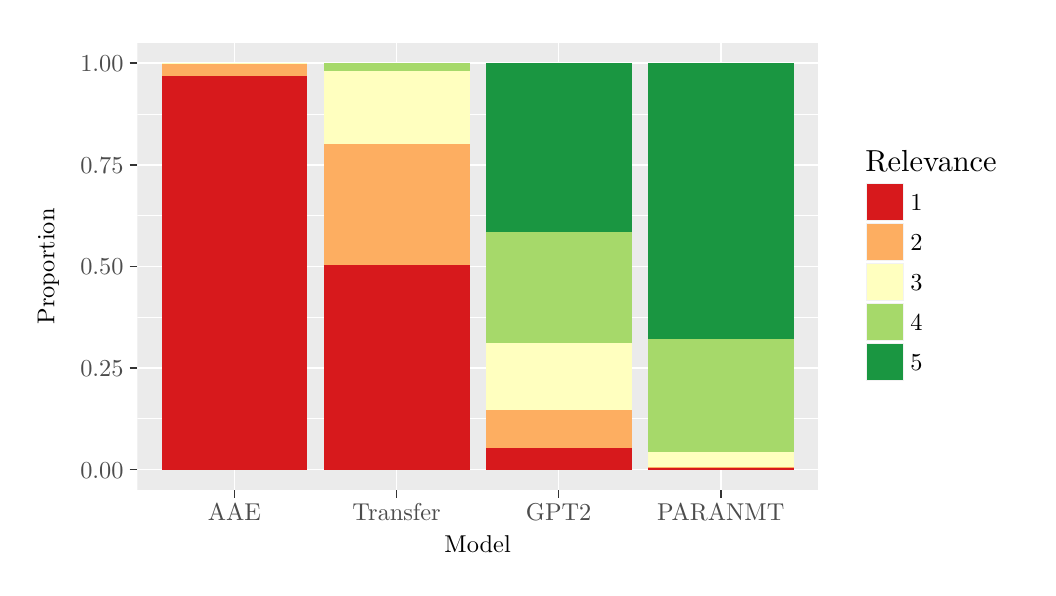
\begin{tikzpicture}[x=1pt,y=1pt]
\definecolor{fillColor}{RGB}{255,255,255}
\path[use as bounding box,fill=fillColor,fill opacity=0.00] (0,0) rectangle (361.35,195.13);
\begin{scope}
\path[clip] (  0.00,  0.00) rectangle (361.35,195.13);
\definecolor{drawColor}{RGB}{255,255,255}
\definecolor{fillColor}{RGB}{255,255,255}

\path[draw=drawColor,line width= 0.6pt,line join=round,line cap=round,fill=fillColor] (  0.00,  0.00) rectangle (361.35,195.13);
\end{scope}
\begin{scope}
\path[clip] ( 39.60, 28.07) rectangle (285.59,189.63);
\definecolor{fillColor}{gray}{0.92}

\path[fill=fillColor] ( 39.60, 28.07) rectangle (285.59,189.63);
\definecolor{drawColor}{RGB}{255,255,255}

\path[draw=drawColor,line width= 0.3pt,line join=round] ( 39.60, 53.77) --
	(285.59, 53.77);

\path[draw=drawColor,line width= 0.3pt,line join=round] ( 39.60, 90.49) --
	(285.59, 90.49);

\path[draw=drawColor,line width= 0.3pt,line join=round] ( 39.60,127.21) --
	(285.59,127.21);

\path[draw=drawColor,line width= 0.3pt,line join=round] ( 39.60,163.93) --
	(285.59,163.93);

\path[draw=drawColor,line width= 0.6pt,line join=round] ( 39.60, 35.42) --
	(285.59, 35.42);

\path[draw=drawColor,line width= 0.6pt,line join=round] ( 39.60, 72.13) --
	(285.59, 72.13);

\path[draw=drawColor,line width= 0.6pt,line join=round] ( 39.60,108.85) --
	(285.59,108.85);

\path[draw=drawColor,line width= 0.6pt,line join=round] ( 39.60,145.57) --
	(285.59,145.57);

\path[draw=drawColor,line width= 0.6pt,line join=round] ( 39.60,182.29) --
	(285.59,182.29);

\path[draw=drawColor,line width= 0.6pt,line join=round] ( 74.74, 28.07) --
	( 74.74,189.63);

\path[draw=drawColor,line width= 0.6pt,line join=round] (133.31, 28.07) --
	(133.31,189.63);

\path[draw=drawColor,line width= 0.6pt,line join=round] (191.87, 28.07) --
	(191.87,189.63);

\path[draw=drawColor,line width= 0.6pt,line join=round] (250.44, 28.07) --
	(250.44,189.63);
\definecolor{fillColor}{RGB}{215,25,28}

\path[fill=fillColor] ( 48.38, 35.42) rectangle (101.09,177.84);
\definecolor{fillColor}{RGB}{253,174,97}

\path[fill=fillColor] ( 48.38,177.84) rectangle (101.09,181.99);
\definecolor{fillColor}{RGB}{255,255,191}

\path[fill=fillColor] ( 48.38,181.99) rectangle (101.09,182.29);
\definecolor{fillColor}{RGB}{215,25,28}

\path[fill=fillColor] (106.95, 35.42) rectangle (159.66,109.44);
\definecolor{fillColor}{RGB}{253,174,97}

\path[fill=fillColor] (106.95,109.44) rectangle (159.66,152.97);
\definecolor{fillColor}{RGB}{255,255,191}

\path[fill=fillColor] (106.95,152.97) rectangle (159.66,179.62);
\definecolor{fillColor}{RGB}{166,217,106}

\path[fill=fillColor] (106.95,179.62) rectangle (159.66,182.29);
\definecolor{fillColor}{RGB}{215,25,28}

\path[fill=fillColor] (165.52, 35.42) rectangle (218.23, 43.11);
\definecolor{fillColor}{RGB}{253,174,97}

\path[fill=fillColor] (165.52, 43.11) rectangle (218.23, 57.03);
\definecolor{fillColor}{RGB}{255,255,191}

\path[fill=fillColor] (165.52, 57.03) rectangle (218.23, 81.02);
\definecolor{fillColor}{RGB}{166,217,106}

\path[fill=fillColor] (165.52, 81.02) rectangle (218.23,121.29);
\definecolor{fillColor}{RGB}{26,150,65}

\path[fill=fillColor] (165.52,121.29) rectangle (218.23,182.29);
\definecolor{fillColor}{RGB}{215,25,28}

\path[fill=fillColor] (224.09, 35.42) rectangle (276.80, 36.01);
\definecolor{fillColor}{RGB}{253,174,97}

\path[fill=fillColor] (224.09, 36.01) rectangle (276.80, 36.30);
\definecolor{fillColor}{RGB}{255,255,191}

\path[fill=fillColor] (224.09, 36.30) rectangle (276.80, 41.93);
\definecolor{fillColor}{RGB}{166,217,106}

\path[fill=fillColor] (224.09, 41.93) rectangle (276.80, 82.79);
\definecolor{fillColor}{RGB}{26,150,65}

\path[fill=fillColor] (224.09, 82.79) rectangle (276.80,182.29);
\end{scope}
\begin{scope}
\path[clip] (  0.00,  0.00) rectangle (361.35,195.13);
\definecolor{drawColor}{gray}{0.30}

\node[text=drawColor,anchor=base east,inner sep=0pt, outer sep=0pt, scale=  0.88] at ( 34.65, 32.38) {0.00};

\node[text=drawColor,anchor=base east,inner sep=0pt, outer sep=0pt, scale=  0.88] at ( 34.65, 69.10) {0.25};

\node[text=drawColor,anchor=base east,inner sep=0pt, outer sep=0pt, scale=  0.88] at ( 34.65,105.82) {0.50};

\node[text=drawColor,anchor=base east,inner sep=0pt, outer sep=0pt, scale=  0.88] at ( 34.65,142.54) {0.75};

\node[text=drawColor,anchor=base east,inner sep=0pt, outer sep=0pt, scale=  0.88] at ( 34.65,179.26) {1.00};
\end{scope}
\begin{scope}
\path[clip] (  0.00,  0.00) rectangle (361.35,195.13);
\definecolor{drawColor}{gray}{0.20}

\path[draw=drawColor,line width= 0.6pt,line join=round] ( 36.85, 35.42) --
	( 39.60, 35.42);

\path[draw=drawColor,line width= 0.6pt,line join=round] ( 36.85, 72.13) --
	( 39.60, 72.13);

\path[draw=drawColor,line width= 0.6pt,line join=round] ( 36.85,108.85) --
	( 39.60,108.85);

\path[draw=drawColor,line width= 0.6pt,line join=round] ( 36.85,145.57) --
	( 39.60,145.57);

\path[draw=drawColor,line width= 0.6pt,line join=round] ( 36.85,182.29) --
	( 39.60,182.29);
\end{scope}
\begin{scope}
\path[clip] (  0.00,  0.00) rectangle (361.35,195.13);
\definecolor{drawColor}{gray}{0.20}

\path[draw=drawColor,line width= 0.6pt,line join=round] ( 74.74, 25.32) --
	( 74.74, 28.07);

\path[draw=drawColor,line width= 0.6pt,line join=round] (133.31, 25.32) --
	(133.31, 28.07);

\path[draw=drawColor,line width= 0.6pt,line join=round] (191.87, 25.32) --
	(191.87, 28.07);

\path[draw=drawColor,line width= 0.6pt,line join=round] (250.44, 25.32) --
	(250.44, 28.07);
\end{scope}
\begin{scope}
\path[clip] (  0.00,  0.00) rectangle (361.35,195.13);
\definecolor{drawColor}{gray}{0.30}

\node[text=drawColor,anchor=base,inner sep=0pt, outer sep=0pt, scale=  0.88] at ( 74.74, 17.06) {AAE};

\node[text=drawColor,anchor=base,inner sep=0pt, outer sep=0pt, scale=  0.88] at (133.31, 17.06) {Transfer};

\node[text=drawColor,anchor=base,inner sep=0pt, outer sep=0pt, scale=  0.88] at (191.87, 17.06) {GPT2};

\node[text=drawColor,anchor=base,inner sep=0pt, outer sep=0pt, scale=  0.88] at (250.44, 17.06) {PARANMT};
\end{scope}
\begin{scope}
\path[clip] (  0.00,  0.00) rectangle (361.35,195.13);
\definecolor{drawColor}{RGB}{0,0,0}

\node[text=drawColor,anchor=base,inner sep=0pt, outer sep=0pt, scale=  0.88] at (162.59,  5.50) {Model};
\end{scope}
\begin{scope}
\path[clip] (  0.00,  0.00) rectangle (361.35,195.13);
\definecolor{drawColor}{RGB}{0,0,0}

\node[text=drawColor,rotate= 90.00,anchor=base,inner sep=0pt, outer sep=0pt, scale=  0.88] at (  9.62,108.85) {Proportion};
\end{scope}
\begin{scope}
\path[clip] (  0.00,  0.00) rectangle (361.35,195.13);
\definecolor{fillColor}{RGB}{255,255,255}

\path[fill=fillColor] (296.97, 61.43) rectangle (355.85,156.27);
\end{scope}
\begin{scope}
\path[clip] (  0.00,  0.00) rectangle (361.35,195.13);
\definecolor{drawColor}{RGB}{0,0,0}

\node[text=drawColor,anchor=base west,inner sep=0pt, outer sep=0pt, scale=  1.10] at (302.66,143.00) {Relevance};
\end{scope}
\begin{scope}
\path[clip] (  0.00,  0.00) rectangle (361.35,195.13);
\definecolor{drawColor}{RGB}{255,255,255}
\definecolor{fillColor}{gray}{0.95}

\path[draw=drawColor,line width= 0.6pt,line join=round,line cap=round,fill=fillColor] (302.66,124.94) rectangle (317.11,139.39);
\end{scope}
\begin{scope}
\path[clip] (  0.00,  0.00) rectangle (361.35,195.13);
\definecolor{fillColor}{RGB}{215,25,28}

\path[fill=fillColor] (303.37,125.65) rectangle (316.40,138.68);
\end{scope}
\begin{scope}
\path[clip] (  0.00,  0.00) rectangle (361.35,195.13);
\definecolor{drawColor}{RGB}{255,255,255}
\definecolor{fillColor}{gray}{0.95}

\path[draw=drawColor,line width= 0.6pt,line join=round,line cap=round,fill=fillColor] (302.66,110.48) rectangle (317.11,124.94);
\end{scope}
\begin{scope}
\path[clip] (  0.00,  0.00) rectangle (361.35,195.13);
\definecolor{fillColor}{RGB}{253,174,97}

\path[fill=fillColor] (303.37,111.19) rectangle (316.40,124.23);
\end{scope}
\begin{scope}
\path[clip] (  0.00,  0.00) rectangle (361.35,195.13);
\definecolor{drawColor}{RGB}{255,255,255}
\definecolor{fillColor}{gray}{0.95}

\path[draw=drawColor,line width= 0.6pt,line join=round,line cap=round,fill=fillColor] (302.66, 96.03) rectangle (317.11,110.48);
\end{scope}
\begin{scope}
\path[clip] (  0.00,  0.00) rectangle (361.35,195.13);
\definecolor{fillColor}{RGB}{255,255,191}

\path[fill=fillColor] (303.37, 96.74) rectangle (316.40,109.77);
\end{scope}
\begin{scope}
\path[clip] (  0.00,  0.00) rectangle (361.35,195.13);
\definecolor{drawColor}{RGB}{255,255,255}
\definecolor{fillColor}{gray}{0.95}

\path[draw=drawColor,line width= 0.6pt,line join=round,line cap=round,fill=fillColor] (302.66, 81.57) rectangle (317.11, 96.03);
\end{scope}
\begin{scope}
\path[clip] (  0.00,  0.00) rectangle (361.35,195.13);
\definecolor{fillColor}{RGB}{166,217,106}

\path[fill=fillColor] (303.37, 82.29) rectangle (316.40, 95.32);
\end{scope}
\begin{scope}
\path[clip] (  0.00,  0.00) rectangle (361.35,195.13);
\definecolor{drawColor}{RGB}{255,255,255}
\definecolor{fillColor}{gray}{0.95}

\path[draw=drawColor,line width= 0.6pt,line join=round,line cap=round,fill=fillColor] (302.66, 67.12) rectangle (317.11, 81.57);
\end{scope}
\begin{scope}
\path[clip] (  0.00,  0.00) rectangle (361.35,195.13);
\definecolor{fillColor}{RGB}{26,150,65}

\path[fill=fillColor] (303.37, 67.83) rectangle (316.40, 80.86);
\end{scope}
\begin{scope}
\path[clip] (  0.00,  0.00) rectangle (361.35,195.13);
\definecolor{drawColor}{RGB}{0,0,0}

\node[text=drawColor,anchor=base west,inner sep=0pt, outer sep=0pt, scale=  0.88] at (318.92,129.13) {1};
\end{scope}
\begin{scope}
\path[clip] (  0.00,  0.00) rectangle (361.35,195.13);
\definecolor{drawColor}{RGB}{0,0,0}

\node[text=drawColor,anchor=base west,inner sep=0pt, outer sep=0pt, scale=  0.88] at (318.92,114.68) {2};
\end{scope}
\begin{scope}
\path[clip] (  0.00,  0.00) rectangle (361.35,195.13);
\definecolor{drawColor}{RGB}{0,0,0}

\node[text=drawColor,anchor=base west,inner sep=0pt, outer sep=0pt, scale=  0.88] at (318.92,100.23) {3};
\end{scope}
\begin{scope}
\path[clip] (  0.00,  0.00) rectangle (361.35,195.13);
\definecolor{drawColor}{RGB}{0,0,0}

\node[text=drawColor,anchor=base west,inner sep=0pt, outer sep=0pt, scale=  0.88] at (318.92, 85.77) {4};
\end{scope}
\begin{scope}
\path[clip] (  0.00,  0.00) rectangle (361.35,195.13);
\definecolor{drawColor}{RGB}{0,0,0}

\node[text=drawColor,anchor=base west,inner sep=0pt, outer sep=0pt, scale=  0.88] at (318.92, 71.32) {5};
\end{scope}
\end{tikzpicture}
